
%%%%%%%%%%%%%%%%%%%%%%% file typeinst.tex %%%%%%%%%%%%%%%%%%%%%%%%%
%
% This is the LaTeX source for the instructions to authors using
% the LaTeX document class 'llncs.cls' for contributions to
% the Lecture Notes in Computer Sciences series.
% http://www.springer.com/lncs       Springer Heidelberg 2006/05/04
%
% It may be used as a template for your own input - copy it
% to a new file with a new name and use it as the basis
% for your article.
%
% NB: the document class 'llncs' has its own and detailed documentation, see
% ftp://ftp.springer.de/data/pubftp/pub/tex/latex/llncs/latex2e/llncsdoc.pdf
%
%%%%%%%%%%%%%%%%%%%%%%%%%%%%%%%%%%%%%%%%%%%%%%%%%%%%%%%%%%%%%%%%%%%


\documentclass[runningheads,a4paper]{llncs}

\usepackage{amssymb}
\setcounter{tocdepth}{3}
\usepackage{graphicx}

\usepackage{url}
\urldef{\mailsa}\path|{alfred.hofmann, ursula.barth, ingrid.haas, frank.holzwarth,|
\urldef{\mailsb}\path|anna.kramer, leonie.kunz, christine.reiss, nicole.sator,|
\urldef{\mailsc}\path|erika.siebert-cole, peter.strasser, lncs}@springer.com|    
\newcommand{\keywords}[1]{\par\addvspace\baselineskip
\noindent\keywordname\enspace\ignorespaces#1}

\begin{document}

\mainmatter  % start of an individual contribution

% TITLE 
\title{ Formalization of Computational Human Behavior Models for Contextual Persuasive Technology }

% SHORT TITLE
\titlerunning{CHBM Formalization}

% the name(s) of the author(s) follow(s) next
%
% NB: Chinese authors should write their first names(s) in front of
% their surnames. This ensures that the names appear correctly in
% the running heads and the author index.
%
\author{Tylar Murray
%\thanks{Please note that the LNCS Editorial assumes that all authors have used
%the western naming convention, with given names preceding surnames. This determines
%the structure of the names in the running heads and the author index.}%
\and Eric Hekler
\and Donna Spruijt-Metz
\and\\ Daniel E. Rivera
\and Andrew Raij
}

% SHORT TITLE (AGAIN)
\authorrunning{CHBM Formalization}
% (feature abused for this document to repeat the title also on left hand pages)

% the affiliations are given next; don't give your e-mail address
% unless you accept that it will be published
\institute{University of South Florida, Arizona State University, University of Southern California, University of Central Florida\\
%Tiergartenstr. 17, 69121 Heidelberg, Germany\\
%\mailsa\\
%\mailsb\\
%\mailsc\\
%\url{http://www.springer.com/lncs}}
tylarmurray@mail.usf.edu
}

%
% NB: a more complex sample for affiliations and the mapping to the
% corresponding authors can be found in the file "llncs.dem"
% (search for the string "\mainmatter" where a contribution starts).
% "llncs.dem" accompanies the document class "llncs.cls".
%

% TODO: WHAT ARE THESE?
\toctitle{Lecture Notes in Computer Science}
\tocauthor{Authors' Instructions}
\maketitle

\begin{abstract}
In theory, Just-in-Time Adaptive Interventions (JiTAIs) are a persuasive technology which promise to empower personal behavioral goals by optimizing treatments to situational context and user behaviors.
In practice, development of a JiTAI represents a major feat which will require integration of several emerging research areas and collaboration between behavioral scientists, systems engineers, and software designers.
This paper outlines open challenges facing the development of JiTAIs and discusses the use of modeling as a common ground between behavioral scientists designing interventions and software engineers building applications.
We propose that Computational Human Behavior Modeling (CHBM) has the potential to 1) help create better behavioral theories, 2) enable real-time ideographic intervention optimization, and 3) facilitate more robust data analysis techniques.
First, a small set of definitions are presented to clarify ambiguities and mismatches in terminology between these two areas.
Next, existing modeling concepts are used to formalize a modeling paradigm designed to fit the needs JiTAI development methodology.
Last, potential benefits and open challenges of this modeling paradigm are highlighted through examination of the model-development methodology, run-time user modeling, and model-based data analysis.

\keywords{
  persusasive, just-in-time, adaptive, JiTAI, modeling, computational human behavior modeling
}
\end{abstract}

%%%%%%%%%%%%%%%%%%%%%%%%%%%%%%%%%%%
%%% %%% %%% PAPER START %%% %%% %%%
%%%%%%%%%%%%%%%%%%%%%%%%%%%%%%%%%%%
\section{Introduction}
A recent trend in the area of persuasive technology is the development of mHealth applications which aim to deliver better, smarter, and more effective interventions via mobile and wearable devices. 
One class of persuasive technologies with this aim is the ``Just-In-Time Adaptive Intervention'' (or JiTAI) which describes an intervention that adapts to an individual's changing needs and circumstances to deliver tailored support at the time when it is most needed. \cite{nahum2014jitais}
Thanks to great advances in wearable, mobile, and ubiquitous technologies increasingly rich data is now available to characterize the context of the subject for use in JiTAI applications.

Researchers theorize that an intervention which can tailor based on the user and context may be an elegant solution to empower self-management of unhealthy behaviors like substance abuse, overeating, sedentary behavior, and more \cite{nahum2014}.
These persuasive technologies aim to utilize contextual information --- data collected from the subject's surroundings and history --- to deliver personalized interventions at the optimal moment in time.
Real-time monitoring of data to identify states of special vulnerability to poor behavioral decisions or receptivity to intervention at any given moment is possible \cite{hekler2013realizing}, but ``a major gap exists between the technological capacity to deliver JITAIs and existing health behavior models.'' \cite{nahum2014}
Proof-of-concept applications have demonstrated the ability to adapt interventions to users \cite{dallery2014optimizing} \cite{beck2010challenges} and context \cite{brailsford2010towards} \cite{collins2004conceptual}, but using current methods the complexity of the behavioral model underlying a JiTAI application grows exponentially as the complexity of the intervention design increases. 
Current methods for conceptualizing the human system take a piece-wise, descriptive approach, examining a phenomena in detail, but often overlooking how the model fits into the bigger picture.
The needs of a persuasive technology are very different from the needs of extant behavioral research.
While the latter places emphasis on the study of the human system's intricacies, the former needs a model which provides generalized insight and specific numerical predictions.
Behavioral theories traditionally focus on nomothetic and static insights that do not offer the granularity and specificity to support the full potential of JiTAIs\cite{riley2011healthbehavior}.
These methods are sufficient for analysis of traits which do not change much over days or weeks, but data collection and intervention delivery timing is now available to the microsecond for physiological data, behavioral features at the minute-level, and psychological constructs (via EMA\cite{shiffman2008ecological}).

The current development process for JiTAI-like persuasive technologies requires close collaboration between behavioral scientists and application developers as they struggle to code-ify the model from extant behavioral theories for each individual experiment.
The models used by a programmer to describe a \emph{user} and the models used by behavioral scientists to describe a \emph{subject}, have certain key differences which can complicate the process of JiTAI design.
In this work we present a hybridization of the two modeling paradigms designed to emphasize the strengths of each approach.

The following interdisciplinary language and concepts will help enable communication between developers and behavioral scientists, and these concepts will also form the foundation of an improved methodology for the development of persuasive technology interventions.
As a part of this set of interdisciplinary terms, we introduce the concept of a Computational Human Behavior Model (CHBM) to describe this new class of models which aim to satisfy the demands of persuasive technology.

Following definitions, we propose that by formalizing the CHBM underlying persuasive applications, it will be possible to create better behavioral theories, enable real-time ideographic optimization, facilitate more robust data analysis, and reduce application development time. 
In this section we present a look at how the concept of a CHBM would be applied to address open issues holding back JiTAIs and we highlight the remaining issues which must be addressed to make Just-in-Time Adaptive Interventions a reality.

\section{Selected Definitions}
% TODO: remove quotes and paraphrase+cite instead?

This section presents definitions and design considerations relevant to human-behavior modeling from a theory-agnostic standpoint so that different modeling paradigms can be described under a common foundation.
This set of definitions draws from both the area of HCI user-modeling and the extant paradigms of human behavior modeling in behavioral science in an attempt to synthesize a pragmatic language for use in the development of persuasive technology by behavioral scientists and application developers alike.

\paragraph{Treatments} are defined by M.C. Kaptein \cite{kaptein2015formalizing} as the set of messages or feedback a user receives from a persuasive application. 
The term treatments seems synonymous with interventions in usage, but a single treatment should be used to unambiguously represent a single instance of user-interaction, whereas a single intervention may represent a set of interactions given as a dose.

\paragraph{Just-in-Time (JiT)} is a cross-disciplinary concept defined in the context of behavioral interactions by Nahum-Shani et al. as ``the effective provision of timely support, operationalized by offering the type of support needed, precisely when needed, in a way that minimizes waste (i.e., defined as anything that does not benefit the person) and accommodates the real-life setting in which support is needed.'' \cite{nahum2014}
Thus, for an intervention to be considered Just-in-Time (JiT), it must attempt to deliver treatment immediately before or after an event associated with the target behavior. 
%For example, a smoking cessation JiT intervention may deliver an intervention in response to increased craving.
%It is important to note here that the term \emph{event} is used to represent any exact set of circumstances over any predefined length of time.
%The targeted event can therefore represent not only \emph{behavioral events} (such as a jog, smoking a cigarette, commuting to work), but also an interval of availability, a ``meaningful moment'', or any ``optimal time'' defined by a match between a set of observed datapoints and a set of datapoints which define the event archetype.

\paragraph{Adaptive} interventions must utilize dynamic (time-varying) ``information from the person (e.g., changes in psychological distress, response to an intervention, intervention adherence) [...] to make intervention decisions repeatedly in the course of the intervention (e.g., changing the type, dosage, or timing of intervention delivery).' \cite{nahum2014}
An adaptive intervention is one that responds in real-time to the changing needs of the participant by tailoring the treatment itself based on situational context or the recent behavioral history of a user. 
%For example, a weight loss trial might attempt to remove soda from a participant's diet and then move on to the next goal if the intervention was successful.
%Similarly, consider the use of step goals to increase physical activity for an obese individual --- the goals may start off at a realistic level (1000 steps/day) and then build up slowly as the individual's ability progresses.

\paragraph{Individualization} is defined by Nahum-Shani et al. as the ``use of [static] information from the individual to make decisions about when, where and how to intervene.'' \cite{nahum2014}
Thus, an intervention is individualized if ``relatively stable information from the person (e.g., gender, baseline severity of symptoms) is used to make intervention-related decisions (e.g., to offer intervention package A or B)'' \cite{nahum2014}
For example, a stress-relief intervention regimen may utilize relaxing music treatment based on the subject's favorite songs at study initialization, or a participant's favorite color may be used as the basis for the user interface color palette.

%\paragraph{Human Behavior Models} (HBMs) are the user models underlying the design of persuasive interventions.
%HBMs can be implicitly or explicitly defined.
%An \emph{implicit} model is one that is expressed through the behavior of the designed system. 
%For instance, an intervention which delivers eating-behavior guidelines daily at noon has an implicit user model which states that users are %awake and likely to eat soon at midday.
%The intervention design reveals the underlying model.
%In contrast, an \emph{explicit} model  defines the user model underlying the operating principles of the intervention. This model is often based on the operationalization of a particular theory (or theories) which have guided the design of the intervention.

\section{Computational Human Behavior Models}
The following specification will allow for the formal description of a CHBM, providing a standard approach to describing, designing, and visualizing human behavior models for persuasive applications.
A Computational Human Behavior Model (CHBM) is defined here as a mathematical, explicit model which describes how context is transformed into a behavioral outcome through the internal state of the human system.
In summary, a Computational Human Behavior Model (CHBM) should have 1) a set of context, state, and behavior variables, 2) a set of computations which define behavior variables as a function of state which is itself a function of context, 3) a logical abstraction which allows researchers to internalize the model's behavior such that they will be better able to estimate control of the human system in general, and 4) guidelines regarding the applicable population and time-scale of the CHBM.
%(i.e. in what populations is the CHBM most/least valid, and at what time-scale can the CHBM simulate realistic predictions?).
The following section details each of these CHBM components, followed by a methodology which makes use of a graph representation to create and describe a particular CHBM.

\subsection{Characteristics of a CHBM}
\subsubsection{User Features: Context, State, Behavior}
A distinguishing feature of a CHBM is the separation of the subject definition into environmental \emph{context}, internal \emph{state}, and \emph{behavior} variables.
In reality, an individual represents an inseparable component within the larger environment, but this simplification segments out the human system for definition.

%Dey et al (2001) performed an extensive literature search to define an agent's context as: ``any information that can be used to characterize the situation of entities (i.e., whether a person, place, or object) that are considered relevant to the interaction between a user and an application, including the user and the application themselves. Context is typically the location, identity, and state of people, groups, and computational and physical objects.''
In most cases, it is sufficient to define context as a set of selected information from the environment available for inflow into the human system, but contextual information from the environment may be summarized and represented in countless ways.
In reality, consider context to be everything that is observed by the senses. 
Some of this information will alter the internal state of the human system, but some may not. 
The selection and summary of contextual data will depend both on the nature of the persuasive system and the data which is available during the experiment.
%The set of internal state variables which define the inner workings of the human system are dependent only on past states and the current context. 
The environmental context influences the human system, which has an internal state represented by a set of internal state variables.
In reality, internal state includes all information stored in the chemical and physical arrangement of our bodies. 
In order to make the model tractable, the mass of information is summarized into a set of meaningful constructs.
%Behavior can be defined in many ways, but in a CHBM behavior is defined as any flow of information out of the human system and into the environment.
Information flowing into a CHBM comes from the environment around an individual (the context) as an inflow which is independent of the individual's state in this instant.
Similarly, information flowing out of a CHBM (as behaviors) represents actions the individual is taking to impact the environment.

\subsubsection{Relationships Between User Features}
The relationships between context, state, and behavior variables in a CHBM must be defined computationally.
The functional form of these computations is not constrained in this definition, theoretically allowing for the representation of any intervariate relationship.
There are numerous benefits to keeping the functional form of these relationships simple and homogenous across variables.
Last, a simple formulation is more easily understood, allowing for a straightforward interpretation and abstraction of the model behavior.

\subsubsection{Heuristic Interpretation}
Statistical models trained on data do qualify as CHBMs in that they can define the relationships between state and context, but typically do not incorporate a logical abstraction of cognition and instead treat the internal state as a \emph{black box}.
This abstraction is essential when considering the process of JiTAI design, since the search-space available to a JiTAI designer can only be approached through heuristics guided by an understanding of how the human system will generally behave under given conditions.
%The interpretation of computational relationships between variables in general terms provides nomothetic insights researchers can use to forecast user behavior without the aid of a simulation.
Though mathematical equations themselves reveal the nature of the system, naming and describing the interpretation of specific constructs or coefficients which play pivotal roles in the model can aid in the process of internalizing model behavior.

\subsubsection{Model Metadata}
While a CHBM should strive to be as broadly applicable as possible, this inevitably comes at the cost of increased complexity which can make the CHBM's nomothetic abstraction(s) intractable; there is a balance to be struck between a CHBM's inclusivity and the clarity of the abstraction.
For this reason, it may be important to specify the circumstances in which a given model is valid.
%It may be useful to craft a highly detailed model of a particular population, but the added complexity in this model may not justify its use in a more general population.
This is not analogous to the issue of over-fitting in machine learning, as the model can remain accurate across the population; the primary reason for limiting the number of variables or the functional complexity of relationships is to preserve the heuristic understanding of the model.

\subsection{Creating a CHBM}
A network graph is an effective abstraction to describe the relationships between nodes in a CHBM.
In this case a directed graph wherein edge arrows represent the flow of information between nodes is used.
Thus, a directed graph edge from node A to node B indicates that information flows from node A into node B. 

\begin{equation}
  A => B
  \label{eq:simplest-sample}
\end{equation}

This relation can be read as ``A influences B'', ``A informs B'', or similar.  
This choice of notation is in agreement with graphs used in information theory, communications models, and behavioral science.
In contrast, some graphing paradigms (such as probabilistic graphical models and software design) prefer to use notation wherein an edge is used to represent dependency.

While the network graph shows the connectivity of a model, it fails to indicate the meaning of each connection.
In the majority of existing applications, the mathematical form of the relationship is implied or else it is neglected completely.
%For instance, path diagrams from the behavioral sciences frequently denote causal dependence and do not specify the functional form of the causal relationship.
%Adding even further to the confusion is the notion that these graphs are often developed using different statistical analyses which may make other assumptions about the functional definition of inter-variate dependency.
The most common analyses assess linear relationships between variables, and thus it is perhaps reasonable to assume that this is the intention of most authors.
Assuming this is the case we can return to our simplistic example in Graph 1 and interpret the implied relationship as:

\begin{equation}
    B(t) = coeff_{ab}A(t) + const_b
    \label{eq:linear-formula}
\end{equation}

In this formulation $coeff_{ab}$ represents the correlation coefficient which relates A to B, and $const_b$ represents a scalar constant.
For nodes with multiple inflow edges, such as node B in the following graph:

\begin{equation}
    A => B <= C => D
    \label{eq:less-simple-graph}
\end{equation}

Continuing with our our assumption that node interrelations act as linear sums, the resulting formulation is simply a sum of the inflows:

\begin{equation}
    B(t) = coeff_{ab}A(t) + coeff_{cb}C(t) + const_b
    \label{linear-formulation}
\end{equation}

%Combining multiple inflows via sum is referred to as the superposition principle and is the defining characteristic of linear systems (not to be confused with this linear formulation).
Using this formulation, the general form of the CHBM is expressed via the network graph alone.
The general solution of an CHBM does not require definition of the constants, but a simulation cannot be run until some numerical value is assumed. 
These constants often have theoretical significance in that they often have meaningful influence upon system behavior. 
Scaling-coefficients, for instance allow for relative weighting of each inflow. 
Similarly, the coefficients of a dynamical equation define how quickly variables react to a change ``upstream''.
%To express an ideographic implementation of this general model, a table of coefficient values must also be included. 

This linear, homogeneous-graph representation is useful, but also very limited.
One important feature which this formulation does not take into account is the dynamics of the relationship.
For instance, the above linear model assumes that there is no delay between variables.
This assumption is fine for some applications, but this is a very poor assumption for human behavior models. 
%What if A is influenced by B but there is some lag before the effect manifests?
%What if A is influenced by B, but only if B is above some threshold value? 
%What if A is influenced by the rate of change in B rather than the value of B itself? 
%All of these scenarios cannot be expressed using this simple linear relationship. 

Differential equations based on a fluid-flow analogy can be used to describe the relationship between variables as described by Dong et al.\cite{dongrivera2012dynamical}. 
Using the differential formulation our equation for B in Graph 1 becomes:

\begin{equation}
    B(t) = coeff_{ab}A(t-\theta_{ab}) - \tau_{b}\frac{dB}{dt} + const
    \label{fluid-flow-eq}
\end{equation}

Just as before, our general model is not expressed entirely through the graph, and an  ideographic example is specified by providing table of coefficient values.
Our table is now quite a bit larger, but these coefficients have meaningful definitions which relate to our theory.
While this formulation offers a huge improvement over the linear formulation, we can still imagine relationships which it cannot express.

It should be noted at this point that although the linear formulation is too simple to express the dynamics of the differential formulation, the differential formulation is capable of expressing linear relationships.
This is accomplished by setting coefficients of dynamical components to 0.
One might think, then, that there is some general formula which could express any functional form, and that this form should be used to express the relationships between variables in all CHBM graphs.
While such formulations do exist (such as Taylor or Fourier series approximations or even ANN-based relations), this usage tends to make the model difficult to understand and to simulate with.
Linear and differential formulations are in such widespread use because of the relative ease with which we can understand and solve them. 
Additionally, the table of coefficients needed to express an idiographic case of the model quickly becomes prohibitively large, and the effect of each coefficient on the outcome is not intuitively meaningful.

Let us now consider the case where a graph-wide assumption is \emph{NOT} made.
That is, we will specify the functional form of each node individually so that each edge on the graph may be linear in form while another may be differential.
This has the benefit of allowing for both complex relationships between variables as well as simplistic ones.
In this way one could craft a model in which two variables are linearly related and a third is dependent on the variance of another variable (a particularly odd formulation, but one which is relevant to behavioral theory).
Unfortunately, this approach also means that a table of formulations must now be included with our graph to show the meaning of each edge in the graph.
Consider for example the table below for Graph 2:

\begin{centering}
  \begin{tabular}{ | l | l | l |}
      \hline
      node & formulation \\ \hline
      B & $coeff_{ab}A(t) + coeff_{cb}C(t) + cosnst_b$  \\ \hline
      D & $coeff_{cd}C(t-\theta_{cd}) - \tau_{d}\frac{dD}{dt} + const_d$ \\ \hline
  \end{tabular}
%Table 1: an example formulation table for Graph 2, showing a linear and first-order differential equation relations between constructs, respectively.
\end{centering}

If a fixed number of functional forms is adhered to, the graph can be made to visually represent these functional forms through the use of different node icon shapes. 
This approach quickly begins to resemble applications which use flow-based programming. 
Indeed, they are quite similar in their approach, and the specification of a CHBM is quite similar to the writing of a program.

Note also that a node can set any arbitrary formulation if needed. 
This is the least desirable situation, since the meaning of an inflow to each node even more convoluted. 
Though this usage reduces the ability of the graph to reduce processing load on the user through abstraction, there may be some cases where this type of formulation is desirable. 
%Consider the following graph and formulation table:
%\begin{equation}
%    A => B <= C => D => E
%\end{equation}

%\begin{centering}
%  \begin{tabular}{ | l | l | l |}
%      \hline
%      node & formulation \\ \hline
%      B & $coeff_{ab}A(t) + coeff_{cb}sqrt(C(t)) + const_b$ \\ \hline
%      D & $coeff_{cd}C(t-\theta_{cd}) - \tau_{d}\frac{dD}{dt} + const_{d}$ \\ \hline
%      E & $coeff_{de}D(t) + const_{e}$ \\ \hline
%  \end{tabular}
%  %Table 2: an example formulation table for Graph 3 showing a custom, differential, and linear relationships, respectively.
%\end{centering}
In conclusion, we propose that an CHBM should be specified using the following rules 1) use a graph-wide formula assumption if possible, else specify formulations for each node individually, 2) when choosing a formulation, consistency between nodes is most important, 3) when choosing a formulation, simplicity and clarity is second only to consistency.
  
%In conclusion, a CHBM specification must include (at minimum) 1) an information flow graph 2) either a graph-wide formulaic assumption or a formulation table.

%\begin{figure}[!t]
%  \centering
%  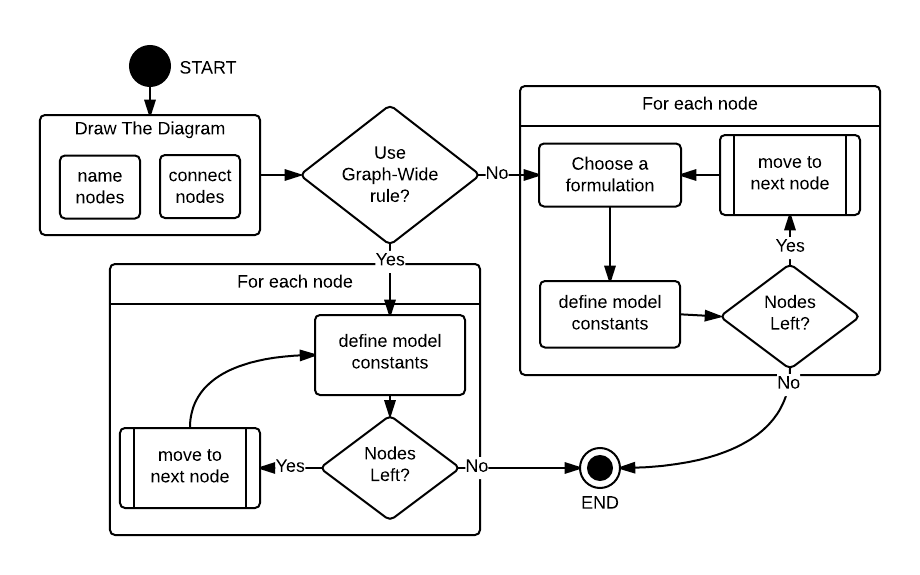
\includegraphics[width=0.9\columnwidth]{img/HBM-build-process}
%  \caption{Flow chart depicting the process of building a graphical CHBM.}
%  \label{HBM-build-process}
%\end{figure}

%It is important to note that the process of building a CHBM is pseudo-linear; users will likely want to jump back to an arbitrary point and as the model takes shape. 
%As the user moves through the process, they will re-assess the meaning of variables and connections and their model will solidify. 

\section{benefits of CHBM-enabled JiTAIs}
This section discusses the utility of a CHBM throughout the lifecycle of a JiTAI application.
Hypothetical situations are posed to highlight the potential value of CHBM use in the JiTAI development process and show open challenges through establishment of a target user group model, application design, application implementation, data analysis, model personalization, and model iteration.
%Existing methods for modeling behavior change are limited in their utility for the average software developer, but a mathematical formulation of the human system's behavior allows developers to utilize existing methods from other engineering domains.

\subsection{\emph{A Priori} CHBMs}
Prior to development of a JiTAI, a mental model of the target user group is established.
This a priori model represents the researcher's understanding of the user group, and the design of the intervention utilizes the model in order to predict user actions.
This level of detail to which this model is documented varies greatly between applications, and in some cases the causal descriptive model has little grounding in existing behavioral theory \cite{prestwich2014does}.
% research has (NOT?) indicated that persuasive applications with a firm basis in theory have been found to be more effective \cite{???}.
% “Establishing a scientific model is an important step in constructing behavioral interventions (Collins, Murphy, and Bierman, 2004).” \cite{nahum2014}
Nevertheless, a vague description of expected user behaviors and interactions with the persuasive technology still represents a user model.
Existing JiTAI-like applications may not have a CHBM, but they always (sometimes informally) imply a CHBM.
This section highlights the benefits of defining a CHBM explicitly, rather than relying on implicit behavioral theory.
\paragraph{Model Building}
When model-building for a JiTAI, the planned system and underlying model of human behavior becomes very complicated, and user responses may be difficult to predict through thought experiments.
Without a concrete framework to describe the model, user behavior becomes oversimplified, giving an even less accurate picture of the complex human system.
When a model is under-developed, the application development process will open unaddressed questions and simple assumptions will be made.
For instance, delivery of a treatment may be limited to the waking hours or to the weekdays, but this will not be reflected in the described user model.
The mismatch between the documented theoretical model and the actually implemented model further muddle the process of study replication and analysis.

In addition to those assumptions knowingly made by application developers, causal descriptive modeling often contains implicit assumptions which are easily overlooked.
For instance, the delay between a cause and effect is frequently neglected --- that is: how quickly does a participant's behavior respond to an treatment?
The process of defining a more detailed a priori model itself can lead to new insights and research questions by eliminating these oversights and forcing critical thinking on the assumptions being made.

% TODO: expand on how dynamical modeling yields insights/research questions: 
% The use of these interventions, particularly in context, forces far more careful description of exactly when, where, and how an intervention might produce an effect and, equally as important, exactly when, where and how an intervention will NOT produce an effect. We might intentionally ask for “outside of the skin” factors such as times, locations, situations and internal states that dictate the boundary conditions on when a  particular causal relationship will be observable or not (Hovell, Wahlgren, and Adams, 2009).  We might also need to discriminate on different “within the skin” attributes that would also define success such as gender, ethnicity, preferences (e.g., while research is increasingly exploring the utility of consuming protein from insects, cultural issues and individual differences make this solution for reducing our collective carbon footprint almost impossible to implement with some groups; Hovell et al. 2009).  These discriminations become even more important when time is taken into account as behavior, “outside the skin” and “inside the skin” factors can all vary together over time (Hovell et al. 2009). This results in clear discrimination of the boundary conditions on when an intervention might work or not, or perhaps only manifest after achieving some largely critical “tipping point,” or wear off after habituation, can further be specified and thought through (Resnicow and Page, 2008; Hekler, et al 2016).

% Beyond the discriminations, there are also a wide range of irrelevant factors that can vary that will not influence the cause and effect relationship(s) under study. It might be believed, for example, that a particular intervention will work the same for men and women.  If that is the case, then having both women and men in the study is useful information  as it supports examining if this “irrelevancy” is truly irrelevant.  

\paragraph{Intervention Design}
When designing intervention options for a JiTAI application, researchers will consider how a treatment influences the subject in the context of the chosen user model.
When using a CHBM, this means quantifying the treatment's effect on user context.
For instance, consider an intervention which provides information about the health repercussions of sedentary behavior.
Assuming our CHBM uses an adaptation of the Theory of Planned Behavior \cite{ajzen1991theory}, this intervention targets \emph{behavioral belief} regarding sedentary behavior.
Since behavioral belief is part of the internal state and the treatment should be defined as part of the user's context, a context variable should be included in our model to represent external influences on behavioral belief from the environment.
After defining the expected effect of a single treatment, the CHBM can then be used to predict a detailed account of user response.
The use of simulations such as this in the process of designing controls is well-explored in many other areas, but is nearly unheard of in behavioral science.
This is in part due to the prevalence of abstract causal descriptive models and the novelty of CHBMs, but there remain several important issues highlighted below which have not yet been addressed in this space.

\emph{Benefits of CHBMs in Persuasive Design:}
\begin{enumerate}
    \item By using a CHBM with dynamical equations, the dynamics of relationships between variables can be explicitly described as a part of the model.
    \item The use of an explicit a priori model for intervention design helps researchers formulate research questions and design experiments in a concrete, testable fashion.
    \item This additional detail needed to define a CHBM removes post-design modeling assumptions and overlooked details that can dilute the underlying behavioral theory or invalidate study results.
    \item The process of defining a CHBM itself can lead to new insights and research questions which are of particular interest to JiTAI design and are almost entirely unaddressed by existing theory.
\end{enumerate}

\emph{Open Questions for CHBM-Empowered Persuasive Design:}
\begin{enumerate}
    \item The process of defining a CHBM requires detailed knowledge of both the underlying behavioral theory and the mathematics. Relatively few researchers today possess the necessary skillset, especially when considering the use of dynamical systems equations.
    \item Modeling software to provide abstraction of the mathematical complexity exists for other engineering domains, but software is not directly applicable to the problem of CHBM development. %TODO how?
    \item Software for running simulations to test the function of an \emph{a priori} CHBM is non-existent, and standards for describing models, simulations, and results in this domain are not established.
    \item Methodologies for creating an \emph{a priori} CHBM are not fully established, and mappings from existing causal descriptive models may be model-dependent.
    \item The definition of an treatment's effect on a user is a subjective process of quantifying qualities which currently have no point of reference.
That is: how is one to know what amount of behavioral belief a specific ``sedentary activity fact treatment'' imparts?
%Guidelines for estimating these values should become more clear after further precedent has been set, but no standards yet exist.
  \item %The running of a single simulation implies a generically applicable user model, but there are likely to be multiple different responses to a single treatment which may depend on on other contextual variables. 
In order to get a more realistic look at user responses to an treatments, many simulations with varying parameters set to match the expectations of the researchers should be run and analyzed; this would require a CHBM simulation software suite that does not yet exist.
\end{enumerate}


\subsection{CHBMs at Run-time}
In this section methods in which CHBMs may be used in the persuasive technology itself are discussed. 
Options include model-based intervention optimization, timing, and online ideographic modeling.

% the trouble with decision rules
A crucial step in the development of a persuasive technology today is to establish a set of \emph{decision rules} based on behavioral theory which codify the circumstances in which a treatment should or should not be delivered.
For instance, a treatment might be delivered only during the daytime, right before a meal, only in a particular location, or in response to a behavioral event such as cigarette use.
Establishing a set of decision rules for a small number of conditions is feasible for a simple intervention, but as the number of conditions increases the number of rules required increases combinatorially.
Even worse, when making use of adaptive interventions this set of rules must be expanded even further to map between all possible contexts and intervention permutations.
Relying on simple decision rules loosely guided by existing theory to define the optimization of intervention delivery to control a complex system inevitably leads to under-optimized interventions, over-simplified models, and weakened data.
An additional problem with this approach is the use of a binary state (i.e. rule satisfied or not) to optimize delivery over a continuous time.
Consider a decision rule which is coincidentally satisfied for the entire first day of the study, and unsatisfied for the rest of the two-week study:
\emph{Should the treatment be delivered on the first day continuously, on some interval, or randomly spread throughout the first day?
Perhaps no treatment be delivered for the remainder of the two weeks while the rule is not satisfied?
Or some minimum number of treatments per day should be spread randomly or applied at particular times?
Should there be a secondary fallback criterion if the primary rule is not satisfied?}
The rules which govern the behavior in this case become part of the theory underlying the application and are clumsily expressed as decision rules.
In contrast, optimization of treatment delivery using a CHBM can be done algorithmically to minimize the area between the desired and observed target behavior.

%Assuming that a CHBM has been formulated by behavioral scientists prior to implementation of the designed application, the software can directly make use of the CHBM to model the user.
Because CHBMs are computational in nature, prediction of behavior is possible given information about the user's present and future context.
Furthermore, because the behaviors in computational models are quantitative, an application could search available treatment options to find one which produces the ideal amount of a target behavior.
%That is, given three treatment options (A, B, C) with known effect on user context, the model can be run at t+1 for each option, and the optimum result can be chosen.
Methods for model predictive control are a well studied topic of control systems engineering, but many methods cannot be applied to generic formulations.
Without a constrained form to guide optimization, all possible options must be explored with equal feasibility in a brute-force search.
With sufficient computational power this is effective for simple problems, but this approach becomes increasingly infeasible as the number of options and the number of future steps to be considered increase.
If the functional form describing variable relationships is constrained appropriately, however, mathematical optimizations methods can greatly simplify this problem.
Applications of model-predictive control over intervention delivery have been explored for gestational weight gain \cite{dong2013hybrid}, smoking cessation \cite{timms2014hybrid}, and fibromyalgia treatment \cite{deshpande2014optimized} by limiting the functional form of the CHBM specification to a differential equation based on a fluid-flow analogy.
In this way, application creators can implement software utilizing the advanced understanding of behavioral science described by the CHBM, without direct knowledge of the underlying behavioral science.

%Methods of optimizing the timing and adaption of interventions thus far have assumed that the effect of treatments is well known a priori.
%However, real-life users may respond very differently from the generalized model and personal ideographic models are not yet a feasible solution.
%In order to optimize intervention delivery given a set of unknown treatments, an online learning has been proposed \cite{jaimes2015calma}.
%In theory, a similar approach may be capable of producing a ideographic models of subjects which can then be generalized to improve understanding of the behavioral theory.

\emph{Benefits of CHBMs for Persuasive Applications:}
\begin{enumerate}
    \item Using a CHBM enables the use of optimization algorithms instead of decision rules. This change is needed to express the complexity necessary to effectively control target behaviors in the human system.
    \item CHBMs can be adapted to fit a user's needs at run-time, establishing an idiographic model of each subject from the generalized CHBM.
\end{enumerate}

\emph{Open Questions for CHBM-enabled Persuasive Applications:}
\begin{enumerate}
    \item Optimization of intervention delivery can be computationally expensive unless the functional form of modelling is restricted, and it is not yet clear what formulations are most appropriate for behavioral construct relationships.
% ??? more ???
\end{enumerate}

\subsection{CHBMs Post-Study}
Another rising challenge for persuasive technology researchers is the increasing complexity of data analysis methods needed to handle large amounts of ``in the wild'' data.
Techniques designed to simplify construct relationships using statistical inferences between distinct groups of measurements cannot address emerging research questions which span the full spectrum of subject demographics, situational context, and time-scale. 
Contemporary approaches apply data mining and machine learning techniques to fit more advanced models to study data and identify key factors, but findings revealed in these exercises can be difficult to generalize and interpret.
%For example, ``even if empirical evidence suggests that a given factor (e.g., psychological distress) marks state of vulnerability to a specific proximal outcome (e.g., it is highly predictive of poor state coping capacity), there is often insufficient empirical evidence concerning the cut-point of this factor that can inform the selection of one intervention option over another.'' \cite{nahum2014}.
%A shift in behavioral research from a focus on relationships between specific variables under specific conditions towards more generalizable hypotheses seems to have begun. 
%This shift is being ushered in by researchers working with persuasive technologies who are looking for practical applications and easy-to-reproduce models of the human system.
By using a model as the hypothesis of an experiment rather than focusing solely on a particular relationship between two variables in specific conditions, research findings can be generalized more easily to practical persuasive applications.
Methods for evaluating models, rather than evaluating correlation between two variables should be increasingly focused upon in the analysis of behavioral data.
While analysis of correlation between variables looks at the statistical relationship between groups of data points, the evaluation of a model involves comparing the experimental data to the predictions of the model.
%Combining CHBMs with the advances in wearable sensors and mobile technology, models are able to predict behavioral outcomes from detailed contextual information collected in the study.
%TODO: include graphic?
CHBMs can be used with contextual data to produce a time series of expected behavioral outcomes throughout the study.
The simulated ``theoretical data'' can then be directly compared to the ``observed data'' to observe how the theory differs from the reality.
The process of comparing theoretical predictions to empirical data can be repeated with simulations from alternate theories and a goodness-of-fit metric can be used to evaluate the hypothesis against alternatives.
Additionally, unification of existing behavioral models into this common paradigm would enable better collaboration between proponents of different theories.

\emph{Benefits of CHBMs Post-Experiment:}
\begin{enumerate}
    \item Through the use of CHBMs, analysis of experimental data can shift focus from individual construct relationships to a larger view, evaluating the model itself as a hypothesis.
    \item Comparison between different theories can be informed by a comparison of their respective models using a goodness-of-fit metric against empirical data.
    \item The use of CHBMs makes re-use of theory and therefore collaborative improvement on existing theories easier than crafting an entirely new theory --- reversing the existing paradigm which has lead to a dizzying multitude of fragmented theories and sub-theories.
\end{enumerate}

\emph{Open Questions for CHBM Post-Experiment Methods:}
\begin{enumerate}
    \item Methods for fitting a model to experimental data require restrictions on the functional form of the relationships between variables, and the optimum functional form is not yet obvious.
    \item Methods for evaluating the goodness-of-fit between empirical and simulated data exist, but cutting-edge software for exploring the intricacies of data mismatch may be difficult to apply to this use-case.
\end{enumerate}

\section{Conclusion}
In this paper we have offered supporting terminology, the CHBM formalization, and a set of open challenges to promote the interdisciplinary discussion needed to push forward the emerging field of JiTAI engineering.
The progression of behavioral science towards computational modeling has progressed more slowly than in other scientific domains because of the limited amount of detailed, time-intensive contextual and behavioral measures available.
This progression from causal descriptive modeling to causal explanitory modeling and increased mathematical rigor is a natural progression which parallels historical trends in the natural sciences.
Now that behavioral and contextual data is becoming accessible, we should expect to see a similar paradigm shift in the behavioral sciences.
%SOME ARTICLE SOMEWHERE highlights the progression of scientific modeling from casual descriptive models to computational modeling as amount of data available to a domain increases, and the study of human behavior seems to be following this trend. \cite{THAT ONE ARTICLE}
It is our hope that this formative work towards Computational Human Behavior Modeling and the methods highlighted here act as a jumping-off point for others on the forefront of this impending paradigm shift who can use these methods to unlock the power of context-aware persuasive application driven by CHBMs.


%%%%%%%%%%%%%%%%%%%%%%%%%%%%%%%%%
%%% %%% %%% PAPER END %%% %%% %%%
%%%%%%%%%%%%%%%%%%%%%%%%%%%%%%%%%

\begin{thebibliography}{4}

\bibitem{ajzen1991theory} Ajzen, I. The theory of planned behavior. Organizational behavior and human decision processes, 50(2), 179-211. (1991)

\bibitem{beck2010challenges} Beck, C., McSweeney, J. C., Richards, K. C., Roberson, P. K., Tsai, P. F., and Souder, E. : Challenges in tailored intervention research. Nursing outlook, 58(2), 104-110. (2010)

\bibitem{brailsford2010towards} Brailsford, S. C., Desai, S. M., and Viana, J. Towards the holy grail: combining system dynamics and discrete-event simulation in healthcare. In Simulation Conference (WSC), Proceedings of the 2010 Winter (pp. 2293-2303). IEEE. (2010)

\bibitem{collins2004conceptual} Collins, L. M., Murphy, S. A., and Bierman, K. L. A conceptual framework for adaptive preventive interventions. Prevention science, 5(3), 185-196. (2004)

\bibitem{dallery2014optimizing} Dallery, J., and Raiff, B. R. : Optimizing behavioral health interventions with single-case designs: from development to dissemination. Translational behavioral medicine, 4(3), 290-303. (2014)

\bibitem{deshpande2014optimized} Deshpande, S., Nandola, N. N., Rivera, D. E., and Younger, J. W. : Optimized treatment of fibromyalgia using system identification and hybrid model predictive control. Control engineering practice, 33, 161-173. (2014)

\bibitem{dongrivera2012dynamical} Dong, Y., Rivera, D. E., Thomas, D. M., Navarro-Barrientos, J. E., Downs, D. S., Savage, J. S., and Collins, L. M. : A dynamical systems model for improving gestational weight gain behavioral interventions. In American Control Conference (ACC), 2012 (pp. 4059-4064). IEEE. (2012)

\bibitem{dong2013hybrid} Dong, Y., Rivera, D. E., Downs, D. S., Savage, J. S., Thomas, D. M., and Collins, L. M. : Hybrid model predictive control for optimizing gestational weight gain behavioral interventions. In American Control Conference (ACC), 2013 (pp. 1970-1975). IEEE. (2013)

\bibitem{hekler2013realizing} Hekler, E. B., Klasnja, P., Traver, V., and Hendriks, M. : Realizing effective behavioral management of health: the metamorphosis of behavioral science methods. Pulse, IEEE, 4(5), 29-34. (2013)

\bibitem{kaptein2015formalizing} Kaptein, M. C. : Formalizing Customization in Persuasive Technologies. In Persuasive Technology (pp. 27-38). Springer International Publishing. (2015)

%\bibitem{jaimes2015calma} Jaimes, L. G., Llofriu, M., and Raij, A. : Calma, an algorithm framework for mobile just in time interventions. In SoutheastCon 2015 (pp. 1-5). IEEE. (2015)

\bibitem{nahum2014} Nahum-Shani, I., Hekler, E. B., and Spruijt-Metz, D. : Building health behavior models to guide the development of just-in-time adaptive interventions: A pragmatic framework. Health Psychology. (2015)

\bibitem{nahum2014jitais} Nahum-Shani, I., Smith, S. N., Tewari, A., Witkiewitz, K., Collins, L. M., Spring, B., and Murphy, S. : Just in time adaptive interventions (jitais): An organizing framework for ongoing health behavior support. Methodology Center technical report, (14-126). (2014)

\bibitem{prestwich2014does} Prestwich, A., Sniehotta, F. F., Whittington, C., Dombrowski, S. U., Rogers, L., and Michie, S. : Does theory influence the effectiveness of health behavior interventions? Meta-analysis. Health Psychology, 33(5), 465. (2014)

\bibitem{riley2011healthbehavior} Riley, W. T., Rivera, D. E., Atienza, A. A., Nilsen, W., Allison, S. M., and Mermelstein, R. : Health behavior models in the age of mobile interventions: are our theories up to the task?. Translational behavioral medicine, 1(1), 53-71. (2011)

\bibitem{shiffman2008ecological} Shiffman, S., Stone, A. A., and Hufford, M. R. : Ecological momentary assessment. Annu. Rev. Clin. Psychol., 4, 1-32. (2008)

\bibitem{timms2014hybrid} Timms, K. P., Rivera, D. E., Piper, M. E., and Collins, L. M. : A hybrid model predictive control strategy for optimizing a smoking cessation intervention. In American Control Conference (ACC), 2014 (pp. 2389-2394). IEEE. (2014)

%\bibitem{jour} Smith, T.F., Waterman, M.S.: Identification of Common Molecular
%Subsequences. J. Mol. Biol. 147, 195--197 (1981)

%\bibitem{lncschap} May, P., Ehrlich, H.C., Steinke, T.: ZIB Structure Prediction Pipeline:
%Composing a Complex Biological Workflow through Web Services. In: Nagel,
%W.E., Walter, W.V., Lehner, W. (eds.) Euro-Par 2006. LNCS, vol. 4128,
%pp. 1148--1158. Springer, Heidelberg (2006)

%\bibitem{book} Foster, I., Kesselman, C.: The Grid: Blueprint for a New Computing
%Infrastructure. Morgan Kaufmann, San Francisco (1999)

%\bibitem{proceeding1} Czajkowski, K., Fitzgerald, S., Foster, I., Kesselman, C.: Grid
%Information Services for Distributed Resource Sharing. In: 10th IEEE
%International Symposium on High Performance Distributed Computing, pp.
%181--184. IEEE Press, New York (2001)

%\bibitem{proceeding2} Foster, I., Kesselman, C., Nick, J., Tuecke, S.: The Physiology of the
%Grid: an Open Grid Services Architecture for Distributed Systems
%Integration. Technical report, Global Grid Forum (2002)

%\bibitem{url} National Center for Biotechnology Information, \url{http://www.ncbi.nlm.nih.gov}

\end{thebibliography}

\end{document}
